\section{The research question}

The practical question is simple: when the movie becomes brighter during a
burst, how much of that signal belongs to a particular neuron, and how much is a
shared property of the recording or its local neighborhood? This distinction
matters because a visually convincing trace can still reflect neuropil,
illumination, motion, broad recruitment, or several neurons at once.

The current dataset contains four burst intervals and 106 confirmed
neuron--burst observations at 50 coordinate-defined sites. The labels are
sparse positives: a confirmed site is a positive example, but an unlabeled
candidate is not automatically a negative. Consequently, the analysis can
measure recovery of known positives, signal fidelity, spatial localization,
and reproducibility. It cannot estimate full-field precision until a bounded
region receives exhaustive review.

\section{What the pipeline does}

The three displayed stages answer different measurement questions:

\begin{enumerate}
  \item \textbf{Raw fluorescence} preserves the acquired intensity and the
  shared burst waveform.
  \item \textbf{Temporal ICA} applies a frozen six-component delay transform at
  lags 0, 1, 2, 4, 8, and 16 frames. Components 2--5 are combined as the
  residual-energy representation used here.
  \item \textbf{Local standardization} compares that representation with a
  causal local space--time reference. Large output means large signal relative
  to the variability recently observed around that location; it does not mean
  ``probability of being a neuron.''
\end{enumerate}

The representative panels keep the movie and center trace synchronized so that
spatial appearance and temporal behavior can be judged together
(\Cref{fig:overview-cases}). The hero, hard antihero, and seeded random case are
illustrative rather than a performance estimate.

\begin{figure}[p]
  \centering
  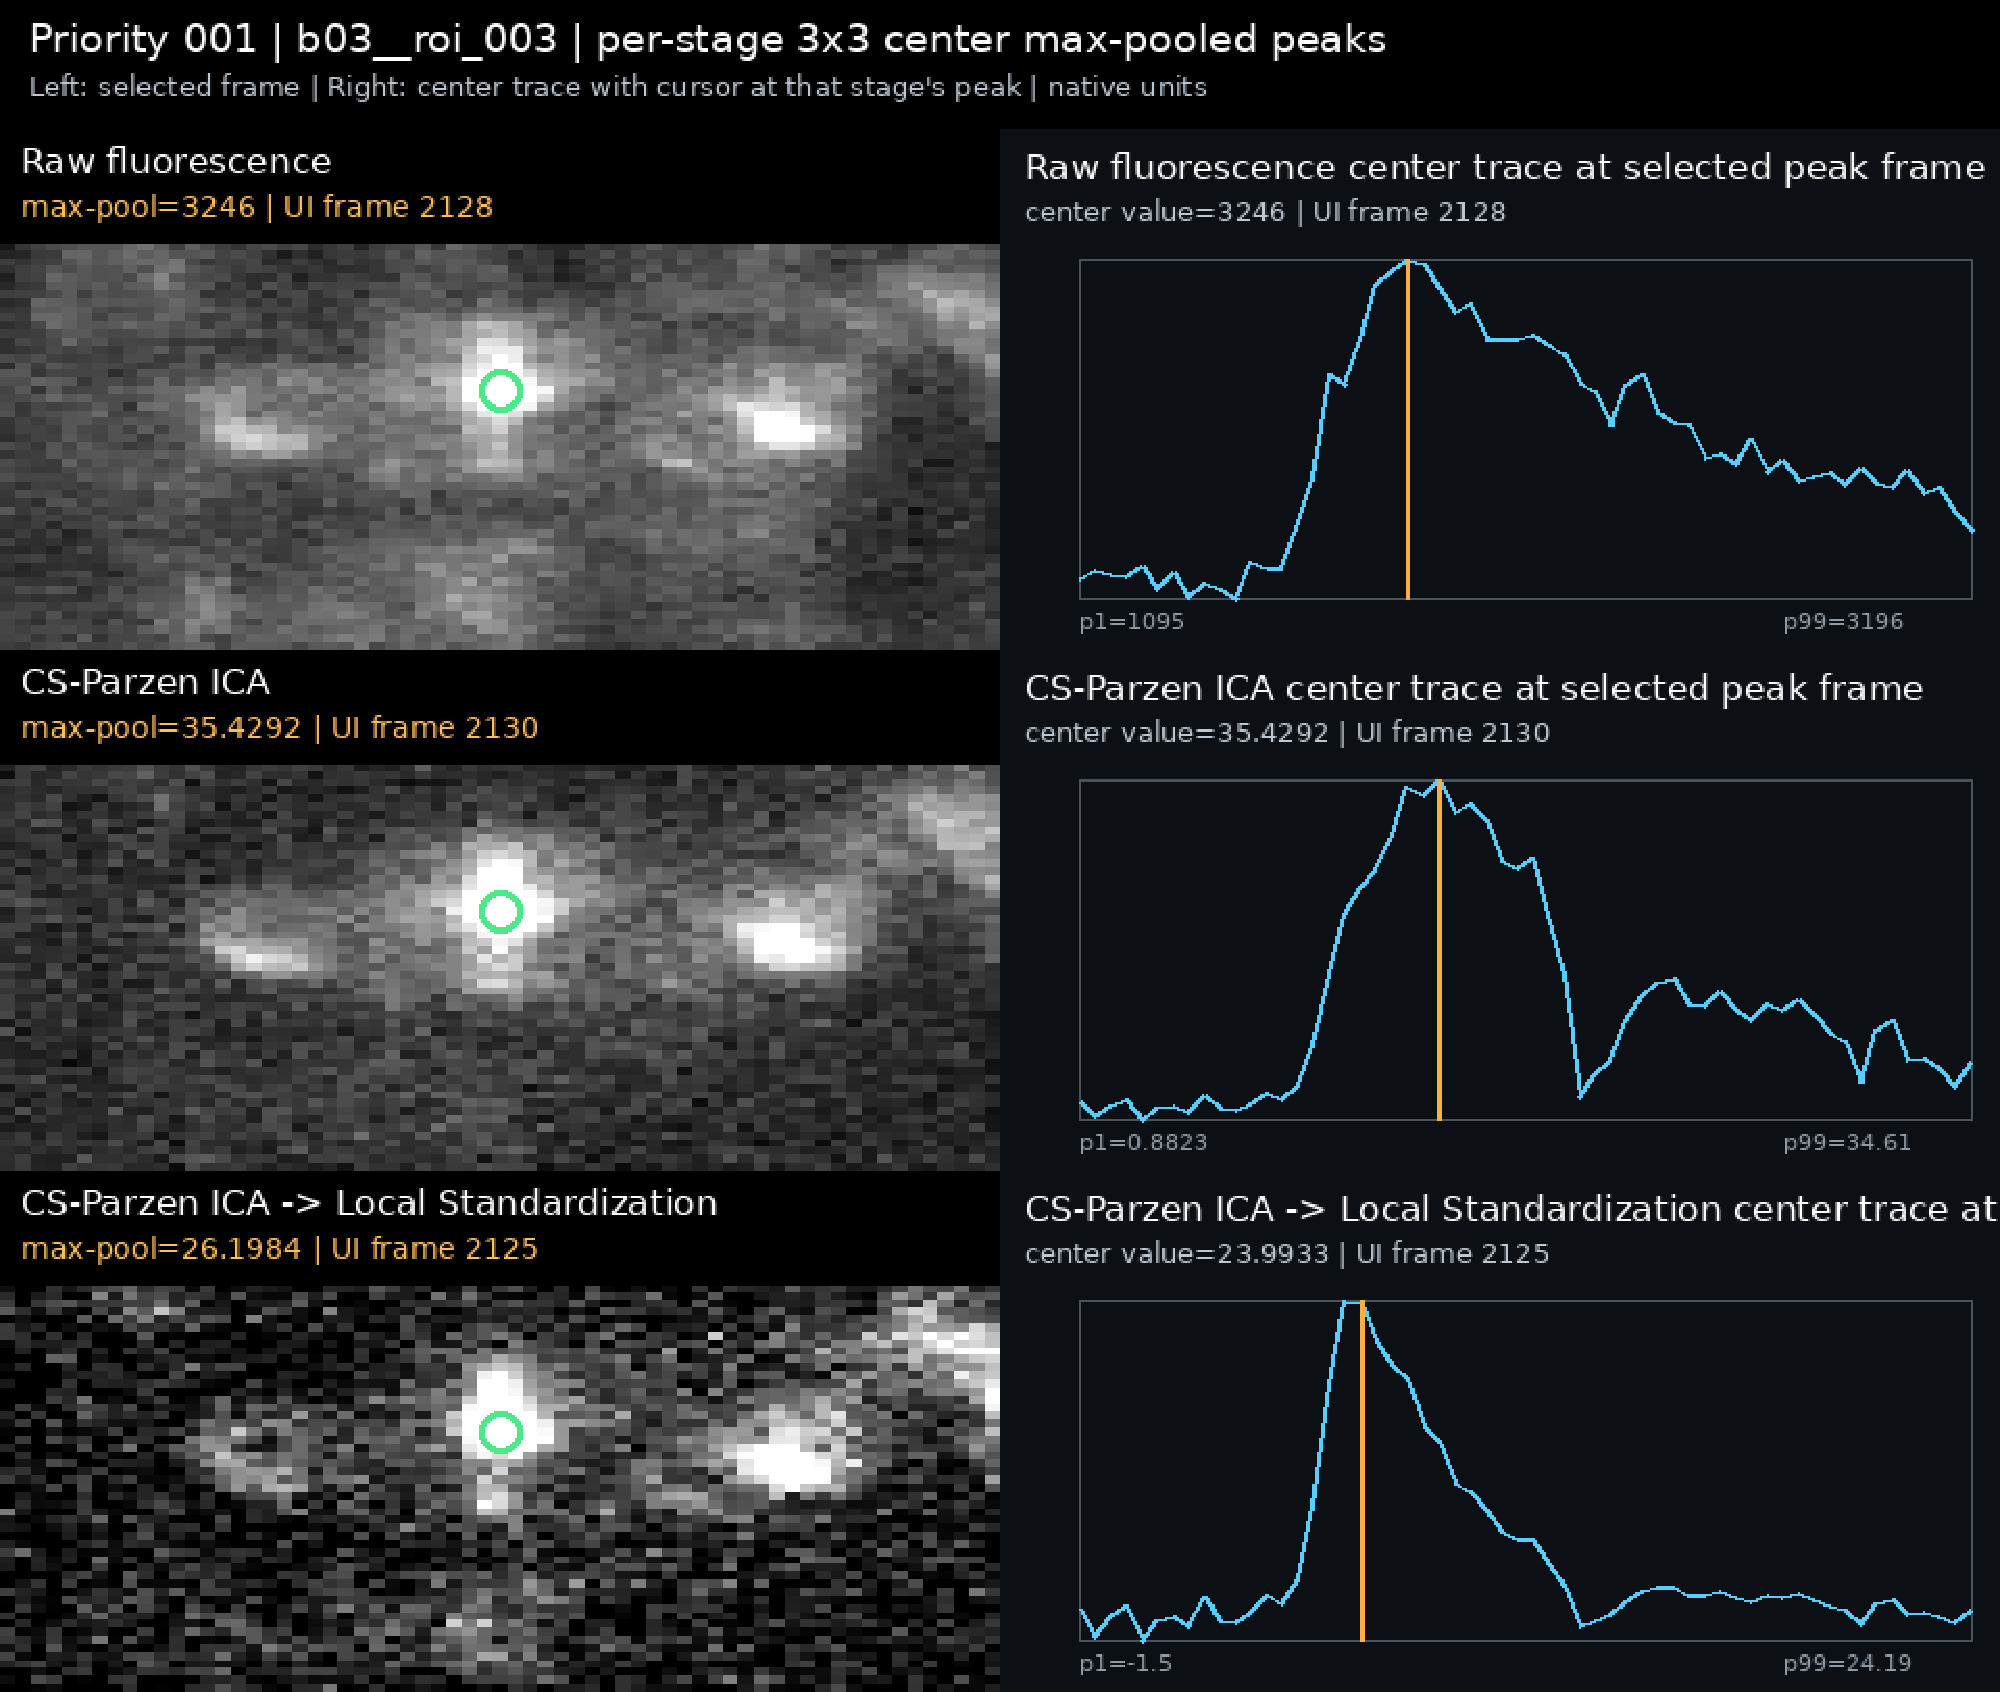
\includegraphics[width=0.96\linewidth,page=1]{figures/final/fig03_trace_atlas_examples.pdf}
  \caption{Representative six-panel review page. Raw, temporal-ICA, and
  local-standardization images are paired with their synchronized ROI-center
  traces. The full technical manuscript includes the hero, antihero, and random
  pages and their frozen selection rules.}
  \label{fig:overview-cases}
\end{figure}
